\documentclass[12pt]{article}
\setlength{\oddsidemargin}{0in}
\setlength{\evensidemargin}{0in}
\setlength{\textwidth}{6.5in}
\setlength{\parindent}{0in}
\setlength{\parskip}{\baselineskip}

\usepackage{amsmath,amsfonts,amssymb,bm,graphics,pgfplots,framed,dsfont}
\usepackage[scale=0.75,top=1cm,bottom=3cm]{geometry}

\begin{document}

\textbf{Minh Anh Nguyen }\\
\textbf{Your class\hfill Your Excersice}

\hrulefill

\begin{enumerate}
      \item Let X be a set with four elements. Represent the identity function $1_X$ of Example 2.22 with a directed graph in two different ways:
      \begin{enumerate}
            \item as an f-graph with four vertices\\
            Let:
                  \[X = \{a,b,c,d\}\]
            The identity function:
            \[X \text{~~~~~~} X\]
            \[a \longrightarrow a\]
            \[b \longrightarrow b\]
            \[c \longrightarrow c\]
            \[d \longrightarrow d\]
            \item with eight vertices, four for the domain and four for the codomain
            Let:\\
                  Domain: \[X = \{a,b,c,d\}\]
                  Codomain: \[Y = \{a,b,c,d\}\]
            \[X \text{~~~~~~} Y\]
            \[a \longrightarrow a\]
            \[b \longrightarrow b\]
            \[c \longrightarrow c\]
            \[d \longrightarrow d\]
      \end{enumerate}

      \item See Definitions 2.3 and 2.4. Write the definitions of one-to-one and onto in terms of predicate logic.\\
      One-to-one definitions in predicate logic:
        \[(\forall x,y \in X)[(f(x) = f(y)) \longrightarrow (x = y)]\]
      Onto definitions in predicate logic:
        \[(\forall y \in Y)(\exists x \in X)[f(x) = y]\]
      \newpage
      \item Show that the function of Example 2.20 is not one-to-one.\\
      Let:
        \[S1 = \{-1,0,1\}\]
        \[S2 = \{0\}\]
      The sum of $S1$ is:
        \[-1 + 0 + 1 = 0\]
      The sum of $S2$ is:
        \[0\]
      \[s(S1) = s(S2) \text{ but } S1 \neq S2\]
      Hence, the function is not one-to-one.
      \item Show that the function of Example 2.20 is onto.\\
      To show the function is onto, for every y there must be \{X\} that the sum of it is y.
      \[y \in Z\]
      and because \{X\} is the set of all nonempty finite sets of integers.
      \[{X} \subset Z\] 
      Hence, we can always choose a set with one value y so:
      \[s(\{y\}) = y\]
      Therefore, the function is onto.
      \item Several languages are spoken in India; let L be the set of all such languages, and let U be the set of all residents of India. Explain why the proposed function f: U → L defined by
            $f(u) = \text{ the language that $u$ speaks.}$
      is not well defined.\\
      Because a person can speaks several languages there can be more than one $f(u)$ with one $u$.\\
      Hence, the function is not well defined.
      \item Let P be a set of people, and let Q be a set of occupations. Define a function f: P → Q by setting f(p) equal to p’s occupation. What must be true about the people in P for f to be a well-defined function?\\~\\
      If f is well defined, for each of the people in P, they must have exactly one occupation in P.
      \item Is the function of Example 2.23 onto? Why or why not? Is it one-to-one? Why or why not?\\
      The function of Example 2.23 is not onto because for all people in P, there are males and females that don't want to give birth.\\
      The function of Example 2.23 is also not one-to-one because there are siblings that have the same birth mothers in P.
      \newpage
      \item Consider Example 2.23. Let y be some person. What is the relationship of $(m \circ m) (y)$ to y?
      \[(m \circ m) (y) = m(m(y))\]
      This means a birth mother of the birth mother of y. Which is y's grandma.
      \item Is the function depicted in Figure 2.8 onto? Why or why not?\\
      \begin{figure}[ht]
            \centering
                 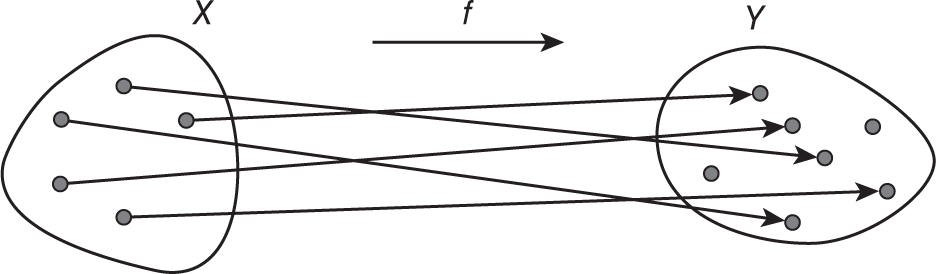
\includegraphics[width=1.0\textwidth]{img/Figure2-8.png}
                  Figure 2.8
                  \label{normal_case}
      \end{figure}\\
      The function depicted in Figure 2.8 is not onto because there 2 y elements in Y that doesn't have any x in X that f(x) = y.
      \item Is the function depicted in Figure 2.9 one-to-one? Why or why not?\\
      \begin{figure}[ht]
            \centering
                 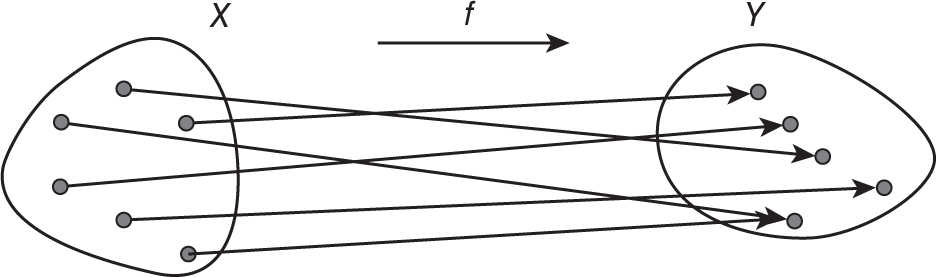
\includegraphics[width=1.0\textwidth]{img/Figure2-9.png}
                  Figure 2.9
                  \label{normal_case}
      \end{figure}\\
      The function depicted in Figure 2.9 is not one-to-one because there are 2 values of x in X with the same y in Y that f(x) = y.
      \item Explain why the proof in Example 2.28 could not be used to prove that the function in Example 2.26 is onto.\\
      Because in Example 2.28, $f:\mathds{R} \longrightarrow \mathds{R}$ so that there will always be an $x$ for $y$ in $\mathds{R}$.
      In Example 2.26, $f:\mathds{Z} \longrightarrow \mathds{Z}$. If y = 6, 2x + 1 = 6 doesn't have any solution in $\mathds{Z}$.
      \item Consider the situation of Example 2.30. Describe a different one-to-one correspondence $g: Y \longrightarrow X$. Show that your function is both one-to-one and onto.\\

\end{enumerate}
\end{document}